\documentclass{beamer}
\usepackage[orientation=portrait,size=a0,scale=1.4,debug]{beamerposter}
\mode<presentation>{\usetheme{CAM}}
\usepackage[utf8]{inputenc}
%\usepackage{siunitx} %pretty measurement unit rendering
\usepackage{hyperref} %enable hyperlink for urls
\usepackage{ragged2e}
\usepackage{calc}
\newlength{\mylength}

\usepackage{array,booktabs,tabularx}
\newcommand{\cE}{\mathcal{E}}                               %
\newcolumntype{Z}{>{\centering\arraybackslash}X} % centered tabularx columns

\title{\huge Viscous Control Of Shallow Elastic Fracture}
\author{Tim Large, John Lister, Dominic Skinner}
\institute[Univerity of Cambridge]
{Department of Applied Mathematics and Theoretical Physics, University of Cambridge}
\date{\today}

\newlength{\columnheight}
\setlength{\columnheight}{105cm}

\begin{document}
\begin{frame}
\begin{columns}
	\begin{column}{.43\textwidth}
		\begin{beamercolorbox}[center]{postercolumn}
			\begin{minipage}{.98\textwidth}  % tweaks the width, 
							%makes a new \textwidth
				\parbox[t][\columnheight]{\textwidth}{ % must bei
% some better way to set the the height, width and textwidth simultaneously
\begin{myblock}{Introduction}
We consider a semi-infinite elastic solid with a thin strip peeled off, and the
resulting crack filled with an incompressible fluid. The motion is driven
by a bending moment applied to the ``arm'' of the solid. The aim is to be
able to write down a set of equations governing the dynamics, in particular
it is of interest to examine the relationship between the speed of traveling
wave solutions $c$, the bending moment $M$, and the toughness 
of the solid $K_I$, $K_{II}$. 

Relevant physical problems include both igneous intrusions beneath a volcano,
and the formation of hydrofractures in an oil
reservoir, since both involve the propagation of a crack through a brittle 
elastic solid driven by fluid injection.

\begin{figure}
\centering\includegraphics[width=0.75\textwidth]{../Fig10.pdf}
\caption{Diagram to show the geometry of the problem. $q(x)$ is the flux,
$g(x)$ the horizontal displacement, $h(x)$ the vertical displacement, and
$\ell$ is the thickness of the arm.}
\end{figure}
\end{myblock}\vfill
\begin{myblock}{Governing Equations}
We assume that the flow everywhere satisfies the lubrication equations. From 
fluid mechanics, we then get the equation
\[12\mu c = h(x)^2 \frac{dp}{dx}.\]

From elasticity, using Muskhelishiveli methods, we can derive the equation
\[
\left[ p,  0 \right]   =
E/(4\pi (1-\nu^2)) \int_0^{\infty}
\textbf{K}(x-\tilde{x}) \;
\left[ g'(\tilde{x}) , h'(\tilde{x}) \right] \, d\tilde{x},  \]
where $K_{ij}$ is the integral kernel specific to this geometry.
\begin{itemize}
\item Boundary conditions as $x\to\infty$ are governed by the bending moment.
      We have (via beam theory), 
      \[ M(x) = \frac{E\ell^3}{12(1-\nu^2)}\frac{d^2h}{dx^2} \to M_0,
        \mbox{ as } x \to \infty. \]
\item The boundary conditions as $x\to0$ are governed by ``\emph{Linear Elastic
      Fracture Mechanics}'', (LEFM). This gives the condition
      \[K_I = \lim_{x\to 0} \; \frac{E}{1-\nu^2}\sqrt{\frac{\pi}{8}} \sqrt{x}
      h'(x), \quad K_{II} = \lim_{x\to 0} \; \frac{E}{1-\nu^2}
      \sqrt{\frac{\pi}{8}} \sqrt{x} g'(x). \]
\end{itemize}
We move into dimensionless variables, 
\[(x,h,g,p,K_I,K_{II},K_{ij},c) \to (\xi, H,G,\Pi, \kappa_{I},\kappa_{II}, 
\Lambda_{ij},\lambda). \]
The new equations and boundary conditions are
\[[\Pi,0] = \int \Lambda \cdot [G',H'] d\xi, \quad H^2\Pi' = \lambda\]
\[\lim_{\xi \to \infty} H'' = 1, \quad \lim_{\xi \to 0} 3\sqrt{2\pi\xi}H' 
= \kappa_I,  \quad \lim_{\xi \to 0} 3\sqrt{2\pi\xi}G' 
= \kappa_{II}. \]
\end{myblock}\vfill
\begin{myblock}{Results}
\begin{figure}
\centering\includegraphics[width=0.95\textwidth]{hprime-p-x-full-poster.pdf}
\caption{Numerical results for two typical $\kappa_I$ values, including
         logarithmic scales for $H'$ and $G'$ (lower two graphs).}
\end{figure}
\end{myblock}\vfill
}\end{minipage}\end{beamercolorbox}
\end{column}
%%%
\begin{column}{.57\textwidth}
\begin{beamercolorbox}[center]{postercolumn}
\begin{minipage}{.98\textwidth} % tweaks the width, makes a new \textwidth
\parbox[t][\columnheight]{\textwidth}{ % must be some better way to set the 
%the height, width and textwidth simultaneously
\begin{myblock}{Small Toughness Solution}
We can plot how the speed $\lambda$ varies with the toughness $\kappa_I$.
For the \emph{small toughness solution}, $\kappa_I \ll 1$, we 
use the theory of Garagash and Detournay \cite{GandD} who consider
fluid driven fracture in a different geometry.
The theory states
\begin{itemize}
\item Near the tip there is the ``LEFM boundary layer''.
\item Away from the tip, the solution behaves as 
      \[H(\xi) = H_0(x) + \cE(\kappa_I)H_1(\xi)+o(\cE),\]
      where $H_0(\xi) = H(\xi ; \kappa_I=0)$ is  the zero toughness solution,
      (similar for $G$,$\Pi$,$\lambda$), and 
      $\cE = C \kappa_I^{u}\lambda_0^{2-u/2}$, $u \approx 3.17$. 
\end{itemize}
This is in good agreement with the numerical results.
\begin{figure}
\centering\includegraphics[width=0.9\textwidth]{l0-poster.pdf}
\caption{The relationship between $\kappa_I$ and $\lambda$ is plotted on the left.
         Strong evidence that $\lambda = \lambda_0 + \cE \lambda_1$, is plotted  
         on the right.}
\end{figure}
\end{myblock}\vfill
\begin{myblock}{Two tip problem}
We can also consider a different mode of fracture. So far, we have been
imposing both a $\kappa_I$ and $\kappa_{II}$ fracture condition at the origin but 
only looking at fracture controlled by the $\kappa_I$ condition. If the 
$\kappa_{II}$ value is small, the solid will fracture by slipping,
and a second dry crack will extend a length $L$ beyond the wet tip. The fracture
is then controlled by the $\kappa_{II}$ value, with the various relationships
plotted in figure \ref{fig:KI0}.
\begin{figure}
\centering\includegraphics[width=0.95\textwidth]{KI-0-poster.pdf}
\caption{These graphs show the interdependence of $L$, $\lambda$ and 
         $\kappa_{II}$, for the two tip problem. Physically $\kappa_{II}$ is
         the independent variable (but not numerically).}\label{fig:KI0}
\end{figure}
Note the (approximately) linear relationship between 
$\kappa_{II}^2$ and $\lambda$. From conservation of energy, and fracture 
mechanics, one expects $\alpha \lambda + \beta
\kappa_{II}^2 = \mbox{ const.}$, where in theory $\alpha$, $\beta$ depend
on $H$, and so $\kappa_{II}$. In practice $\alpha$ and $\beta$ are almost
constant, as seen from the graph.
 
\end{myblock}\vfill
\begin{myblock}{Overall results}
Solving the one tip problem for various $\kappa_I,\kappa_{II}$ values gives
a graph in the $\kappa_I , \kappa_{II}$-plane. From this we can determine where
the fracture is controlled by $\kappa_I$ and where it is controlled by
$\kappa_{II}$. For $\kappa_I > 1.9$ and $\kappa_{II} > 1.5$,
the fracture cannot propagate, the solid is too tough.
\begin{figure}
\centering\includegraphics[width=0.85\textwidth]{catagory-poster.pdf}
\caption{For a given $(\kappa_I, \kappa_{II})$ value, this diagram shows where
         the fracture speed is limited by the $\kappa_I$ or $\kappa_{II}$ value,
         and where there is a two tip fracture.}\label{fig:catagory}
\end{figure}
\begin{figure}
\centering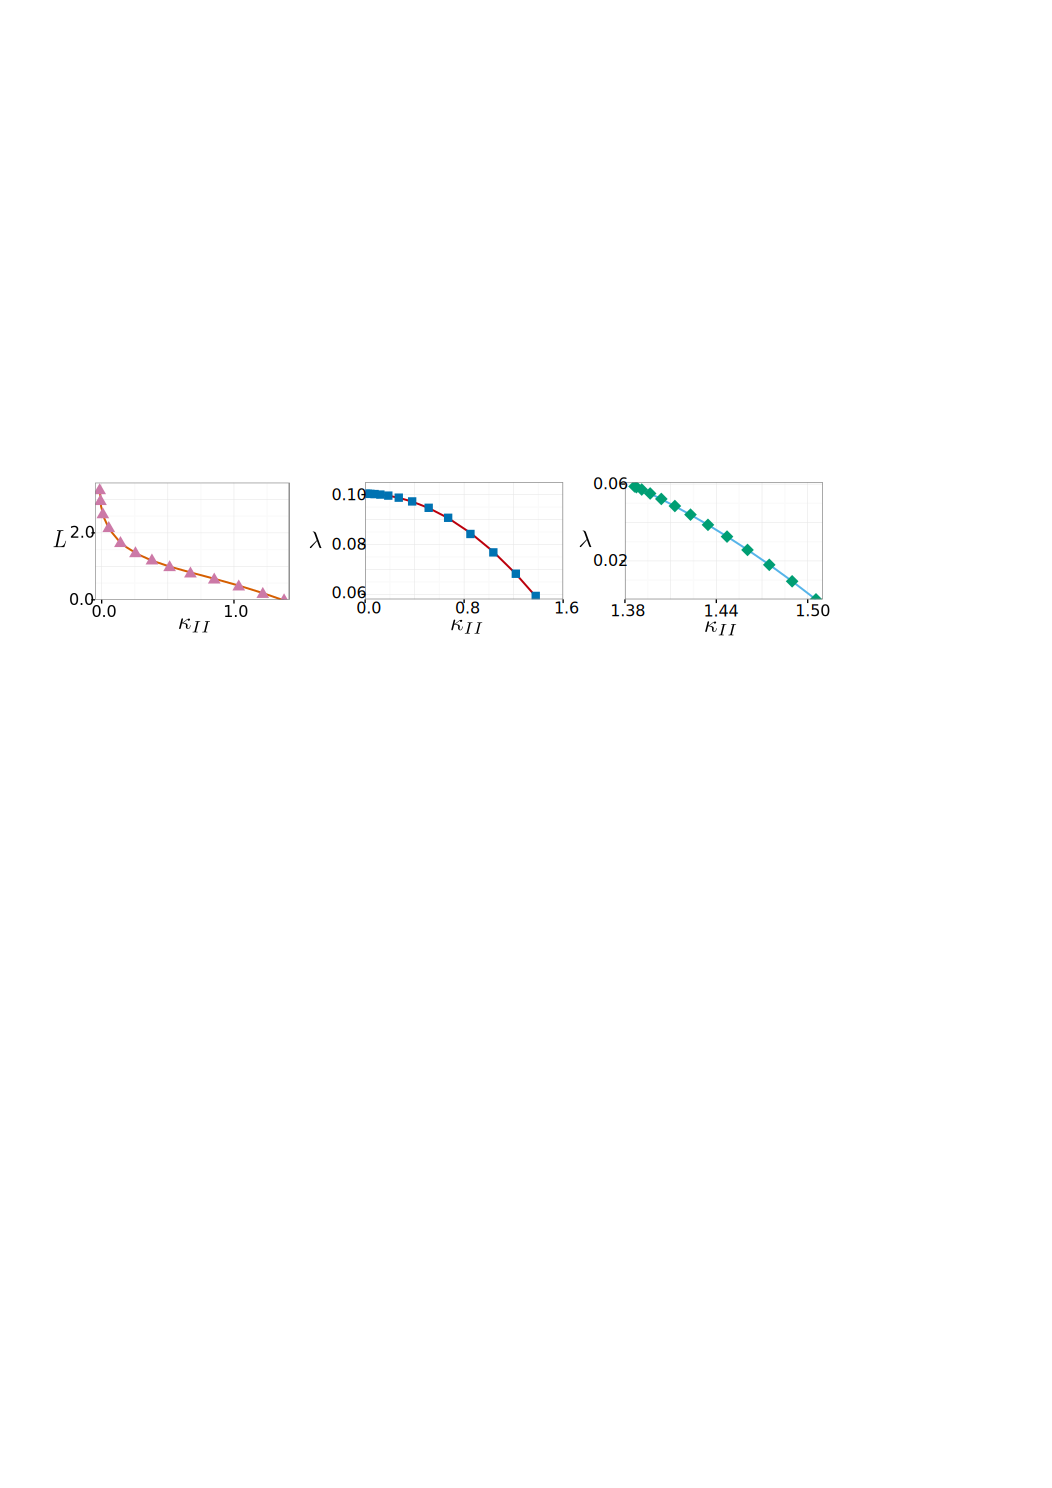
\includegraphics[width=0.95\textwidth]{overall-fit-poster.pdf}
\caption{When the fracture speed is limited by $\kappa_{II}$, these graphs
         provide a way of calculating $\lambda$, $L$ in terms of $\kappa_{II}$.
         The two graphs on the left are for $L>0$ and the graph on the right is
         for $L=0$.}
\end{figure}
\end{myblock}\vfill
\begin{myblock}{References}
\footnotesize
\begin{thebibliography}{9}  
%
\bibitem{GandD}
Garagash, D.I., Detournay, E.,
\emph{Plane-Strain Propagation of a Fluid-Driven Fracture: Small Toughness
Solution,}
Journal of Applied Mechanics,
2005.
%
%
\end{thebibliography}
%\bibliographystyle{unsrt}
%\bibliography{./bib}
\end{myblock}\vfill
}\end{minipage}\end{beamercolorbox}
\end{column}
\end{columns}
\end{frame}
\end{document}

